\documentclass[12pt]{article}
\title{Edzőterem működését támogató szoftver PureScript és Vue.js alapokon}
\author{Mezei Botond, Szabó Benedek}
\date{2023}
\renewcommand{\contentsname}{Tartalomjegyzék}
\usepackage[utf8]{inputenc}
\usepackage{graphicx}
\graphicspath{ {./images/} }
\usepackage{wrapfig}
\renewcommand{\figurename}{Ábra}
\usepackage{amsmath}
\usepackage{subcaption}
\usepackage{amssymb}
\usepackage[export]{adjustbox}
\usepackage[magyar]{babel}
\usepackage[breaklinks]{hyperref}
\usepackage{microtype}
\usepackage[T1]{fontenc}
\usepackage{lmodern}
\usepackage{multirow}
\usepackage[table]{xcolor}
%\usepackage{natbib}

\setlength{\arrayrulewidth}{0.5mm}
\setlength{\tabcolsep}{7pt}
\renewcommand{\arraystretch}{2.5}

\textwidth=14cm \textheight=20cm
%\hoffset=-1cm
%\voffset=-1cm

\newtheorem{theorem}{Theorem}[section]
\newtheorem{acknowledgement}[theorem]{Acknowledgement}
\newtheorem{algorithm}[theorem]{Algorithm}
\newtheorem{axiom}[theorem]{Axiom}
\newtheorem{case}[theorem]{Case}
\newtheorem{claim}[theorem]{Claim}
\newtheorem{conclusion}[theorem]{Conclusion}
\newtheorem{condition}[theorem]{Condition}
\newtheorem{conjecture}[theorem]{Conjecture}
\newtheorem{corollary}[theorem]{Corollary}
\newtheorem{criterion}[theorem]{Criterion}
\newtheorem{definíció}[theorem]{Definíció}
\newtheorem{discussion}[theorem]{Discussion}
\newtheorem{example}[theorem]{Example}
\newtheorem{exercise}[theorem]{Exercise}
\newtheorem{explanation}[theorem]{Explanation}
\newtheorem{illustration}[theorem]{Illustration}
\newtheorem{lemma}[theorem]{Lemma}
\newtheorem{notation}[theorem]{Notation}
\newtheorem{problem}[theorem]{Problem}
\newtheorem{proposition}[theorem]{Proposition}
\newtheorem{remark}[theorem]{Remark}
\newtheorem{solution}[theorem]{Solution}
\newtheorem{summary}[theorem]{Summary}

\makeatletter
%\renewcommand*{\@biblabel}[1]{–}
\makeatother

\begin{document}
\begin{titlepage}

	\begin{center}
	\mbox{}\\
	\vspace{35mm}
	\huge
	\textsc{Diplomamunka}
	\end{center}

	
	\vspace{55mm}
	\Large
	\hspace*{\fill} 
	\textbf{Mezei Botond, Szabó Benedek}
	
	\begin{center}
	\vspace{55mm}
	Debrecen\\	
	2023
	
	\end{center}
\end{titlepage}
\begin{titlepage}

	\vspace*{-2cm}
	\hspace*{-1.5cm}

	\begin{center}
	\large
	Debreceni Egyetem
	
	Informatikai Kar	

	Számítógéptudományi Tanszék
	
	\vspace{17mm}
	\huge
	\LARGE
    \textbf{Edzőterem működését támogató szoftver PureScript és Vue.js alapokon}
	
	\vspace{15mm}
	\large
	\textsc{Diplomamunka}
	
	\normalsize
	\vspace{20mm}
	\textsc{Készítette:}
	
	\vspace{5mm}
	\Large
	\textbf{Mezei Botond és Szabó Benedek}
	
	\normalsize
	programtervező informatika szakos hallgatók
	
	\vspace{18mm}
	\textsc{Témavezető:}\\
	\vspace{5mm}
	\large
	Dr. Battyányi Péter \\
	\normalsize
	adjunktus\\
	
	\vspace{32mm}
	Debrecen\\	
	2023
	
	\end{center}
\end{titlepage}
\newpage
\tableofcontents
\newpage
\section*{Bevezetés}
\addcontentsline{toc}{section}{Bevezetés}

miert ezt valasztottuk

mi a munkánk és a dolgozat célja

A huszonegyedik század harmadik évtizedében minden vállalatnak, cégnek vagy szervezetnek elengedhetetlenül szükségessé vált az informatika bevonása a mindennapi működésbe. A cégek versenyképességük megőrzése, a hatékonyság és profitabilitás növelése érdekében már gyakorlatilag egy mikrovállalkozás méretétől kezdve rászorulnak valamiféle speciális céges szoftver, vállalatirányítási rendszer használatára. Egy kicsit nagyobb vállalatnál pedig már egészen elképzelhetetlen lenne a működés e szoftverek nélkül. A költségcsökkentés és automatizálás mellett meg kell említeni az információ növekvő szerepét, egy vállalatirányítási rendszer biztosíthatja a gyors (valós idejű) információ hozzáférést a munkatársaknak, illetve adatokkal látja el a döntéshozókat.

\newpage
\section{Szakirodalmi áttekintés}

\subsection{Funkcionális programozás}
A funkcionális programozás egy programozási paradigma. Több programozási nyelv is tartozik ide, melyeket bizonyos tulajdonságok, módszereik, lehetőségeik, gondolkodási logikájuk köti össze. Az egyik korai funkcionális nyelv a Lisp, melyet John McCarthy alkotott meg az 1950-es évek végén \cite{JM}. Ismertebb funkcionális nyelvek például Haskell, Elm, Erlang, Scala vagy a PureScript. 
A funkcionális programozás során a fejlesztő azt specifikálja a programban, hogy mit kell kiszámítani, és nem azt, hogy hogyan, milyen lépésekben \cite{VD}. A program függvények hívásából és ezek kiértékeléséből áll, nincs értékadás, csak érték kiszámítás \cite{VD}. A függvényt leginkább úgy értjük, hogy egy leképezés egy adott halmazról egy másik halmazra\cite{sy}. A listák (vagy halmazok) kezelésének ezért kiemelt szerep jut a funkcionális nyelvekben. A program tartalmazhat a nyelvben előre definiált, és a programozó által definiált függvényeket. A függvények névvel és opcionálisan argumentumokkal rendelkeznek. Az előállított érték(ek) megegyező paraméterekkel mindig ugyanaz. A rekurzió egy nagyon gyakori koncepció funkcionális nyelvekben.

Egy másik nagy paradigma az imperatív programozás. Az imperatív nyelvek lényege, hogy a programozó a lépéseket definiálja a kódban, melyet a számítógépnek el kell végeznie (utasítások). A legismertebb imperatív nyelv a C.

A logikai programozási paradigma lényege, hogy a programozó állításokat, szabályokat rögzít, melyek használatával a gép automatikusan kikövetkezteti, hogy egy kérdéses állítás igaz, vagy sem. Ilyen nyelv például a Prolog.

Manapság az egyik legelterjedtebb paradigma az objektumorientált programozás. Ez egy gondolkodásmód, tervezési módszer is egyben. A valós világot osztályok formájára képezi le, melynek egyedeit objektumok személyesítenek meg. Legfőbb elvei az egységbezárás (encapsulation: az adatmodell és az eljárásmodell szétválaszthatatlansága), öröklődés (újrafelhasználhatóság kiterjesztése), hozzáférés-szabályozás és többalakúság (polimorphism: lehetővé teszi, hogy ugyanarra az üzenetre különböző objektumok a saját módjukon válaszoljanak) \cite{VD}.

A ma leginkább használatos nyelvekre általánosságban igaz az, hogy nem csupán egyetlen paradigmát követnek tisztán, hanem többet vegyítenek. Ennek az az oka, hogy minden paradigmának megvan a maga előnye (és persze hátránya is), és ezeket az előnyöket érdemes kihasználni. Például a Java (2023. áprilisában a harmadik legtöbbet használt nyelv \cite{TIO}) alapjaiban imperatív, objektumorientált, de a nyolcas verziótól kezdve \cite{Java} megjelennek benne funkcionális elemek, például a lambda kifejezések. A nyelv hivatalos oldala \cite{Java} "erőteljes kiterjesztés"-nek nevezi ezt a lépést.

\subsubsection{A funkcionális programozás előnyei}
A funkcionális programozás, mint paradigma, számos előnnyel rendelkezik. Az imperatív gondolkodás kötöttségét egy másfajta megközelítéssel oldja fel. A lényeg, hogy \textit{mit} csináljon a program, és nem az, hogy \textit{hogyan}. Ez az ötlet a programozótól is  másfajta megközelítést, gondolkodásmódot kíván, és máshogy strukturált kódot is fog eredményezni. 

Ránézésre jobban érthető, átláthatóbb, esztétikusabb kód. A szoftver "viselkedése" jobban olvasható \cite{CS}. Ez az előny egyszerűen a funkcionális szintaktikából és gondolkodásmódból adódik. A következő Java kódrészletek Boris Radojicic 2022-es cikkéből \cite{sy} származnak. Az elsőn az iteratív megközelítés látható:

\begin{verbatim}
public List<String> getAddresses(List<Person> persons) {
    List<String> addresses = new ArrayList<>();
    for (int i = 0; i < persons.size(); i++) {
        Person person = persons.get(i);
        if (person.hasValidData()) {
            String address = person.getAddress();
            addresses.add(address.trim());
        }
    }
    return addresses;
}
\end{verbatim}
A következő kódrészlet pedig a funkcionális megközelítést alkalmazza:
\begin{verbatim}
public List<String> getAddresses(List<Person> persons) {
    return persons.stream()
            .filter(person -> person.hasValidData())
            .map(person -> person.getAddress())
            .map(address -> address.trim())
            .collect(Collectors.toList());
}
\end{verbatim}
Míg a két kód ugyanazt a viselkedést eredményezi, a kettőre ránézve elmondható, hogy a második olvashatóbb és tömörebb.

Nagy fokú újrafelhasználhatóság. Mivel egy funkcionális program gyakorlatilag függvények deklarálásából és függvényhívásokból áll, ezeket a függvényeket nagy mértékben újra lehet hasznosítani, elkerülve a feleslegesen duplikált kódrészleteket. A felesleges kód rontja az átláthatóságot és több erőforrást is igényel.

Könnyebb tesztelhetőség. Mivel a funkcionális programban nincsenek állapotok és mellékhatások, így könnyebb lefedni az összes esetet. Illetve ebből kifolyóan, a függvénynek bizonyos bemenő paraméterekre mindig ugyanazt az egyértelmű kimenetet kell előállítania.

A rekurzió hatékony használata. A rekurzió a funkcionális nyelvek gyakori eleme. Átláthatóvá és egyértelművé teszi a kódot teszi a kódot bizonyos problémák esetében, ahol a rekurzív definiálás a természetesebb megoldás. A rekurziónak egy speciális esete a farokrekurzió. Ez azt jelenti, hogy a rekurzív hívás a legutolsó művelet, amit a függvény végrehajt. Nagy előnye, hogy idő és erőforrás takarékos a nem farokrekurzív függvényekkel szemben, ugyanis a fordító kevesebb információt kell, hogy tároljon ilyen módon a veremben.

\subsubsection{A funkcionális programozás nehézségei}

Az előnyök között első helyen állt az átláthatóság és érthetőség. Ehhez viszont hozzátartozik az, hogy a fejlesztő előtte megismerje és elsajátítsa a funkcionális programozás gondolkodásmódját, ami néha bizony nem egyszerű és nem a legtermészetesebb megoldásnak tűnhet.

Memóriahasználat és teljesítmény. Mivel a funkcionális nyelvek nem használnak érték-átadást, sokszor egy változó értékének megváltozása helyett létrejön egy újabb, ami így több erőforrást igényel \cite{JN}. A legtöbb funkcionális nyelv ennek ellenére számos módon ígyekszik ezt kompenzálni: farokrekurzió, lusta kiértékelés, "smart linking". A több paradigmát támogató vagy OOP nyelvek nem feltétlen implementálják ezeket az optimalizációkat \cite{JN}.

Mivel a funkcionális nyelvek használata kevésbé elterjedt, kevesebb eszköz, keretrendszer áll rendelkezésre és kevesebb a felhasználók, szakértők száma.

\subsection{PureScript}

A PureScript egy erősen típusos, tisztán funkcionális nyelv. Javascript kódra fordul. Amit Javascriptben meg lehet írni, azt nagyjából PureScriptben is \cite{CS}. A böngészőben és  a szerveren egyaránt futtatható. A Haskell az alapja, sokban hasonlít rá. Charles Scalfani \cite{CS} szerint erősebb, de egyben könnyebben is használható.
Frontend és backend fejlesztésre egyaránt alkalmas lehet \cite{CS}.

\subsection{Vue.js}

\newpage
\section{Eredmények és azok értékelése}

\begin{figure}
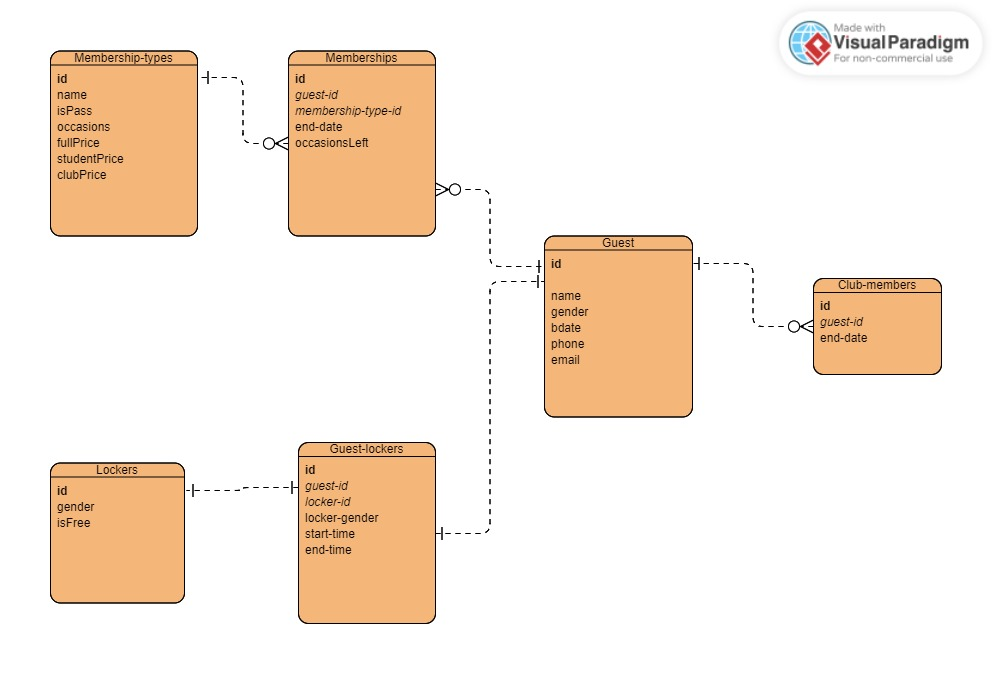
\includegraphics[width=\textwidth]{database}
\caption{A szoftver adatbázis modellje.}
\end{figure}

\newpage
\section{Továbbfejlesztési lehetőségek}

A vizsgált és specifikációk készítésekor használt modellezési nyelvek (ARIS, BPMN, UML, Petri-hálók) közül én az ARIS-t találtam jelen feladathoz a legmegfelelőbbnek. A különböző diagramtípusok integrációja és azok rendszerezett kezelése mindenképp kiemeli a többi közül. Ezen felül leginkább a folyamatok leírásakor az általa kínált információtöbbletet is hasznosnak találtam, véleményem szerint a többinél nagyobb kifejezőerővel rendelkezik ez az eszköz. 

\newpage
\section*{Összefoglalás}
\addcontentsline{toc}{section}{Összefoglalás}

A mai korszerű vállalatoknak versenyképességük megőrzése céljából elengedhetetlenné vált üzleti szoftverek alkalmazása. Dolgozatom célkitűzése egy debreceni kereskedelmi profilú kisvállalkozás folyamatainak, működésének megismerése, modellezése és a számára készülő vállalatirányítási rendszer üzleti követelmény specifikációjának elkészítése volt. 

%******************példa képek:

%\begin{figure}
%\centering
%\includegraphics[width=0.7\textwidth]{org}
%\caption{Organogram.}
%\end{figure}

%\begin{wrapfigure}{r}{0.4\textwidth}
%\includegraphics[width=0.4\textwidth]{test1}
%\caption{Értékteremtő lánc diagram.}
%\end{wrapfigure}

%\begin{figure}[h]
%\centering
%\begin{subfigure}{0.45\textwidth}
%\includegraphics[width=8cm]{pelda1} 
%\end{subfigure}
%\begin{subfigure}{0.4\textwidth}
%\includegraphics[width=8cm]{pelda2}
%\end{subfigure}
%\caption{A háló $t_1$ tüzelése előtt és után}
%\end{figure}

%******************felsorolas
%\begin{definíció}
%A Petri háló ($PN$) egy ($P, T, E, w, m_0$) rendszer, ahol
%\begin{enumerate}
%\item $P$ a helyek véges halmaza,
%\item $T$ a tranzíciók véges halmaza feltéve, hogy $P \cap T = \emptyset$,
%\item $E \subseteq (P \times T) \cup (T \times P)$ az élek véges halmaza,
%\item $ w: E\rightarrow N^+$ a súlyfüggvény,
%\item $ m: P\rightarrow N$ a token-eloszlás függvény,
%\item $ m_0$ a kezdeti token eloszlás.
%\end{enumerate}
%A Petri háló struktúrát $(P, T, E, w)$ módon jelöljük. (\textit{Peterson., 1981})
%\end{definíció}

\addcontentsline{toc}{section}{Irodalomjegyzék}

\newpage
\renewcommand{\refname}{Irodalomjegyzék}
\begin{thebibliography}{99}

\bibitem{CS}
C. Scalfani. Functional Programming Made Easier: A Step-by-Step Guide. 2021.

\bibitem{PE}
P. Freeman. PureScript by Example. 2014 - 2017.
\url{https://book.purescript.org/}

\bibitem{VD}
Dr. Vadász Dénes: Programozási paradigmák, programozási nyelvek (letölthető egyetemi oktatási anyag)
\url{https://web.archive.org/web/20150501083657/http://www.iit.uni-miskolc.hu/iitweb/export/sites/default/users/DVadasz/GEIAL401/Progpar-4-fejezet.pdf#}
Hozzáférés dátuma: 2023.04.11.

\bibitem{JM}
John McCarthy: The implementation of LISP. 1996.
http://www-formal.stanford.edu/jmc/history/lisp/node3.html

\bibitem{Sz}
Szuromi Zs.: Programozási paradigmák, kézirat. ME, 1996.

\bibitem{TIO}
The TIOBE Programming Community index. \url{https://www.tiobe.com/tiobe-index/} Hozzáférés dátuma: 2023.04.11.

\bibitem{Java}
A Java nyelv hivatalos honlapja. \url{https://dev.java/learn/lambdas/}  Hozzáférés dátuma: 2023.04.11.

\bibitem{sy}
B. Radojicic.: Imperative to Functional Programming in Java. 2022
\url{https://symphony.is/blog/imperative-to-functional-programming-in-java} Hozzáférés dátuma: 2023.04.11.

\bibitem{JN}
J. Neumann.: Advantages and disadvantages of functional programming. 2022.
\url{https://medium.com/twodigits/advantages-and-disadvantages-of-functional-programming-52a81c8bf446}
Hozzáférés dátuma: 2023.04.12.

\bibitem{PS}
\url{https://www.purescript.org/}

\bibitem{vue}
\url{https://vuejs.org/guide/introduction.html}

\end{thebibliography}
\end{document}
